\documentclass[a4paper,12pt]{report}
\usepackage[english]{babel}
\usepackage{graphicx}
\usepackage{placeins}
\usepackage{hyperref}
\usepackage{supertabular}
\usepackage{listings}
\usepackage{color}
\lstset{% general command to set parameter(s)
basicstyle=\footnotesize,
keywordstyle=\color{black}\bfseries\underbar,
identifierstyle=\color{black}\bfseries\underbar,
stringstyle=\ttfamily,
}




\title{FoLiA: Format for Linguistic Annotation \\ \small v0.7}
\author{Maarten van Gompel \\ ILK Research Group \\ Tilburg center for Cognition and Communication \\ Tilburg University }

\parindent=0pt %no paragraph indentation
\parskip=12pt %paragraph skip


\newenvironment{devnotes}
{
\begin{center}
    \begin{tabular}[h!]{|p{0.8\textwidth}|}
    \hline
    {\bf Development Notes}\\\hline}
{   \\\hline
    \end{tabular}
\end{center}}

\begin{document}
\sffamily

\maketitle
\tableofcontents


\chapter{Introduction}

FoLiA is a Format for Linguistic Annotation, derived from the D-Coi format\cite{DCOI} developed as part of the D-Coi project by project partner at Polderland Language and Speech Technologies B.V. The D-Coi format was designed for use by the DCOI corpus, as well as by its successor; the SoNaR corpus \cite{Oostdijk+08}. Though being rooted in the D-Coi format, the FoLiA format goes a lot further and introduces a rich generalised framework for linguistic annotation. FoLiA is developed at the ILK research group, Tilburg University, and proposed as a CLARIN standard in the TTNWW project.

FoLiA is an XML-based\cite{XML} annotation format, suitable for representing written language resources such as corpora. Its goal is to unify a variety of linguistic annotations in one single rich format, without committing to any particular standard annotation set. Instead, it seeks to accommodate any desired system or tagset, and so offer maximum flexibility. This makes FoLiA language independent. Due to its generalised set up, it is easy to extent the FoLiA format to suit your custom needs for linguistic annotation.

XML is an inherently hierarchic format. FoLiA does justice to this by maximally utilising a hierarchic, inline, setup. We inherit from the D-Coi format, which posits to be loosely based on a minimal subset of TEI\cite{TEI}. Because of the introduction of a new and broader paradigm, FoLiA is \emph{not} backwards-compatible with D-Coi, i.e. validators for D-Coi will not accept FoLiA XML. It is however easy to convert FoLiA to less complex or verbose formats such as the D-Coi format, or plain-text. Converters will be provided. This may entail some loss of information if the simpler format has no provisions for particular types of information specified in the FoLiA format. 


In contrast to the D-Coi format, the FoLiA format introduces annotation layers separate from the token-based skeleton structure, to capture structured linguistic annotations such as syntactic parses. This is to provide FoLiA with the necessary flexibility and extensibility. Inspiration for this was in part obtained from the Kyoto Annotation Format \cite{KYOTO}. 

The FoLiA format features the following:

\begin{itemize}
\item Open-source
\item XML-based, validation against RelaxNG schema.
\item Full Unicode support; UTF-8 encoded.
\item Document structure consists of divisions, paragraphs, sentences and words/tokens.
\item Can encode both tokenised as well as untokenised text + partial reconstructability of untokenised form even after tokenisation.
\item Support for crude token categories (word, punctuation, number, etc)
\item Explicit support for encoding quotations
\item Provenance support for all linguistic annotations: annotator, type (automatic or manual), time.
\item Support for alternative annotations, optionally with associated confidence values.
\item Adaptable to different tag-sets.
\item Agnostic with regard to metadata. CMDI is recommended, but alternatives like IMDI can also be used.
\end{itemize}

It supports the following linguistic annotations:

\begin{itemize}
\item Part-of-Speech tags (with features)
\item Lemmatisation
\item Spelling corrections on both a tokenised as well as an untokenised level
\item Lexical semantic sense annotation (to be used in DutchSemCor)
\item Named Entities / Multi-word units
\item Syntactic Parses
\item Dependency Relations
\item Chunking
\item Morphological Analysis

\end{itemize}

In later stages, the following may be added:

\begin{itemize}
\item Semantic Role Labelling
\item Co-reference
\item Topic Segmentation
\item Authorship Attribution
\item Subjectivity Annotation (to be used in VU-DNC)
\end{itemize}


FoLiA support will be incorporated directly into the following ILK sofware:

\begin{itemize} 
\item ucto - A tokeniser which can directly output FoLiA XML 
\item Frog - A PoS-tagger/lemmatiser/parser suite (the successor of Tadpole), will eventually support reading and writing FoLIA.
\item CLAM - Computational Linguistics Application Mediator, will eventually have viewers for the FoLiA format.
\item PyNLPl - Python Natural Language Processing Library, will come with libraries for parsing FoLiA
\item libfolia - C++ library for parsing FoLiA
\end{itemize}

FoLiA will be used in the DutchSemCor project, the DU-VNC project, and will also be proposed for consideration in the SoNaR project. It is also proposed as a CLARIN standard in the TTNWW project.

To clearly understand this documentation, note that when we speak of ``elements'' or ``attributes'', we refer to XML notation, i.e. XML elements and XML attributes.

\chapter{Document Format}

\section{Global Structure}

In FoLiA, each document/text is represented by one XML file. The basic structure of such a FoLiA document is as follows and should always be UTF-8 encoded. An elaborate XSLT stylesheet will be provided in order to be able to instantly view FoLiA documents in any modern web browser.

\begin{lstlisting}[language=xml]
<?xml version="1.0" encoding="utf-8"?>
<?xml-stylesheet type="text/xsl" href="http://ilk.uvt.nl/FoLiA/FoLiA.xsl"?>
<FoLiA xmlns="http://ilk.uvt.nl/FoLiA"
  xmlns:xsi="http://www.w3.org/2001/XMLSchema-instance" 
  version="0.5"
  xml:id="example">
  <metadata>
      <annotations>
          ...
      </annotations>    
      <!-- (Here CMDI or IMDI metadata can be inserted) -->
  </metadata>
  <text xml:id="example.text">
     ...
  </text>
</FoLiA>  
\end{lstlisting}



\section{Identifiers}

Many elements in the FoLiA format specify an identifier by which the element is uniquely identifiable. This makes referring to any part of a FoLiA document easy and follows the lead of the D-Coi format. Identifiers should be unique in the entire document, and can be anything that qualifies as a valid ID according to the XML standard. A well proven convention is of a cumulative nature, in which you append the elements name, a period, and a sequence number, to the identifier of a parent element higher in the hierarchy. Identifiers are always encoded in the \texttt{xml:id} attribute. The FoLiA document as a whole also carries an ID.

Identifiers are very important and used throughout the FoLiA format. They enable external resources and database to easily point to a specific part of the document or its annotation. FoLiA has been set up in such a way that \emph{identifiers should never ever change}. Once an identifier is assigned, it should never change, re-numbering is strictly prohibited unless you intentionally want to create a new resource and break compatibility with the old one.

\section{Basic Structural Elements}
\label{sec:basics}

Basic structural elements occur within the \texttt{text} element. These are the most basic ones:

\begin{itemize}
\item \texttt{p} - Paragraph
\item \texttt{s} - Sentence
\item \texttt{w} - Word (token)
\end{itemize}

These are typically nested, the word elements cover the actual tokens. This is the most basic level of annotation; tokenisation. Let's take a look at an example, we have the following text:

\begin{verbatim}
This is a paragraph containing only one sentence.

This is the second paragraph. This one has two sentences.
\end{verbatim}

In FoLiA XML, this will appear as follows after tokenisation. Some parts have been omitted for the sake of brevity:


\begin{lstlisting}[language=xml]
 <p xml:id="example.p.1">
    <s xml:id="example.p.1.s.1">        
        <w xml:id="example.p.1.s.1.w.1"><t>This</t></w>
        <w xml:id="example.p.1.s.1.w.2"><t>is</t></w>
        ...
        <w xml:id="example.p.1.s.1.w.8" space="no"><t>sentence</t></w>
        <w xml:id="example.p.1.s.1.w.9"><t>.</t></w>
    </s>
 </p>
 <p xml:id="example.p.2">
    <s xml:id="example.p.2.s.1">
        <w xml:id="example.p.2.s.1.w.1"><t>This</t></w>
        <w xml:id="example.p.2.s.1.w.2"><t>is</t></w>    
        ..
        <w xml:id="example.p.2.s.1.w.5" space="no"><t>paragraph</t></w>    
        <w xml:id="example.p.2.s.1.w.6"><t>.</t></w>    
    </s>
    <s xml:id="example.p.2.s.2">
        <w xml:id="example.p.2.s.2.w.1"><t>This</t></w>
        <w xml:id="example.p.2.s.2.w.2"><t>one</t></w>    
        ..
        <w xml:id="example.p.2.s.2.w.5" space="no"><t>sentences</t></w>    
        <w xml:id="example.p.2.s.2.w.6"><t>.</t></w>    
    </s>
 </p>
\end{lstlisting}


The deepest content element should always contain a text element (\texttt{t}) which holds the actual textual content. The necessity of having a text element shall become apparent as you progress through this documentation; there can be many different token annotations under a word element (\texttt{w}).

FoLiA is not just a format for holding tokenised text, although tokenisation is a prerequisite for almost all kinds of annotation. However, FoLiA can also hold untokenised text, on a paragraph and/or sentence level:

\begin{lstlisting}[language=xml]
 <p xml:id="example.p.1">
    <s xml:id="example.p.1.s.1">        
        <t>This is a paragraph containing only one sentence.</t>
    </s>
 </p>
 <p xml:id="example.p.2">
    <s xml:id="example.p.2.s.1">     
        <t>This is the second paragraph.</t>
    </s>
    <s xml:id="example.p.2.s.2">     
        <t>This one has two sentences.</t>
    </s>    
 </p>
\end{lstlisting}

Higher level elements \emph{may} also contain a text element even when the deeper element does too. It is very important to realise that the sentence/paragraph-level text element \emph{always} contains the text \emph{prior} to tokenisation! Note also that the word element has an attribute \texttt{space}, which defaults to yes, and indicates whether the word was followed by a space in the \emph{untokenised} original. This allows for partial reconstructibility of the sentence in its untokenised form. See section~\ref{sec:textcontent} for a more elaborate overview of this subject.

The following example shows the maximum amount of redundancy, with text elements at every level.

\begin{lstlisting}[language=xml]
 <p xml:id="example.p.1">
    <t>This is a paragraph containing only one sentence.</t>
    <s xml:id="example.p.1.s.1">        
        <t>This is a paragraph containing only one sentence.</t>
        <w xml:id="example.p.1.s.1.w.1"><t>This</t></w>
        <w xml:id="example.p.1.s.1.w.2"><t>is</t></w>
        ...
        <w xml:id="example.sp.1.s.1.w.8" space="no"><t>sentence</t></w>
        <w xml:id="example.p.1.s.1.w.9"><t>.</t></w>
    </s>
 </p>
 <p xml:id="example.p.2">
    <t>This is the second paragraph. This one has two sentences.</t>
    <s xml:id="example.p.2.s.1">
        <t>This is the second paragraph.</t>
        <w xml:id="example.p.2.s.1.w.1"><t>This</t></w>
        <w xml:id="example.p.2.s.1.w.2"><t>is</t></w>    
        ..
        <w xml:id="example.p.2.s.1.w.5" space="no"><t>paragraph</t></w>    
        <w xml:id="example.p.2.s.1.w.6"><t>.</t></w>    
    </s>
    <s xml:id="example.p.2.s.2">
        <t>This one has two sentences.</t>
        <w xml:id="example.p.2.s.2.w.1"><t>This</t></w>
        <w xml:id="example.p.2.s.2.w.2"><t>one</t></w>    
        ..
        <w xml:id="example.p.2.s.2.w.5" space="no"><t>sentences</t></w>    
        <w xml:id="example.p.2.s.2.w.6"><t>.</t></w>    
    </s>
 </p>
\end{lstlisting}

It this kind of redundancy is used (it is not mandatory),you may optionally point back to the text content of its parent by specifying the \texttt{offset} attribute:

\begin{lstlisting}[language=xml]
 <p xml:id="example.p.1">
    <t>This is a paragraph containing only one sentence.</t>
    <s xml:id="example.p.1.s.1">        
        <t offset="0">This is a paragraph containing only one sentence.</t>
        <w xml:id="example.p.1.s.1.w.1"><t offset="0">This</t></w>
        <w xml:id="example.p.1.s.1.w.2"><t offset="5">is</t></w>
        ...
        <w xml:id="example.p.1.s.1.w.8" space="no"><t offset="40">sentence</t></w>
        <w xml:id="example.p.1.s.1.w.9"><t offset="48">.</t></w>
    </s>
 </p>
\end{lstlisting}

Matters can become more complicated as multiple text-content element of different classes may be associated with an element, this will be discussed later on in section~\ref{sec:textcontent}.

Paragraph elements may be omitted if a document is described that does not distinguish paragraphs but only sentences. Sentences however may never be omitted; FoLiA documents can never consist of tokens only!

The content element \texttt{head} is reserved for headers and captions, it behaves similarly to the paragraph element and may hold sentences.

FoLiA also explicitly supports quotes, as demonstrated in the next example, which annotates the following sentence: 

\begin{verbatim}
He said: ``I do not know . I think you are right. ", and left.
\end{verbatim}

A quote may consist of one or more sentences, but may also consist of mere tokens. The token identifiers in all cases simply follow the sequential numbering of the root sentence, not the embedded sentence.


\begin{lstlisting}[language=xml]
 <s xml:id="example.p.1.s.1">
  <w xml:id="example.p.1.s.1.w.1" class="WORD"><t>He</t></w>
  <w xml:id="example.p.1.s.1.w.2" class="WORD"><t>said</t></w>
  <w xml:id="example.p.1.s.1.w.3" class="PUNCTUATION" space="no"><t>:</t></w>
  <w xml:id="example.p.1.s.1.w.4" class="PUNCTUATION" space="no"><t>''</t></w>
  <quote xml:id="example.p.1.s.1.quote.1">
    <s xml:id="example.p.1.s.1.quote.1.s.1">
       <w xml:id="example.p.1.s.1.w.5" class="WORD"><t>I</t></w>
       <w xml:id="example.p.1.s.1.w.6" class="WORD"><t>do</t></w>
       <w xml:id="example.p.1.s.1.w.7" class="WORD"><t>not</t></w>
       <w xml:id="example.p.1.s.1.w.8" class="WORD"><t>know</t></w>
       <w xml:id="example.p.1.s.1.w.9" class="PUNCTUATION" space="no"><t>.</t></w>
    </s>
    <s xml:id="example.p.1.s.1.quote.1.s.2">
       <w xml:id="example.p.1.s.1.w.10" class="WORD"><t>I</t></w>
       <w xml:id="example.p.1.s.1.w.11" class="WORD"><t>think</t></w>
       <w xml:id="example.p.1.s.1.w.12" class="WORD"><t>you</t></w>
       <w xml:id="example.p.1.s.1.w.13" class="WORD"><t>are</t></w>
       <w xml:id="example.p.1.s.1.w.14" class="WORD"><t>right</t></w>
    </s>
  </quote>
  <w xml:id="example.p.1.s.1.w.15" class="PUNCTUATION" space="no"><t>''</t></w>
  <w xml:id="example.p.1.s.1.w.16" class="PUNCTUATION"><t>,</t></w>
  <w xml:id="example.p.1.s.1.w.17" class="WORD"><t>and</t></w>
  <w xml:id="example.p.1.s.1.w.18" class="WORD"><t>left</t></w>
  <w xml:id="example.p.1.s.1.w.19" class="PUNCTUATION" space="no"><t>.</t></w>
 </s>
\end{lstlisting}

\section{Paradigm \& Terminology}
\label{sec:paradigm}

The FoLiA format has a very uniform setup and its XML notation for annotation follows a generalised paradigm. We distinguish three different categories of annotation, of which the latter two apply to actual linguistic annotation:

\begin{itemize}
\item \textbf{Structural annotation} - Annotations marking global structure, such as chapters, sections, subsections, figures, list items, paragraphs, etc...
\item \textbf{Token annotation} - Annotations pertaining to one specific token. These will be elements of the token element (\texttt{w}) in inline notation. Linguistic annotations in this category are for example: part-of-speech annotation, lemma annotation, sense annotation, morphological analysis, spelling correction. Some token elements may be used on higher levels (e.g. sentence/paragraph) as well and may then be referred to as \textbf{Extended Token Annotation}
\item \textbf{Span annotation} - Annotations spanning over multiple tokens. Each type of annotation will be in a separate \textbf{annotation layer} with offset notation. These layers are typically embedded on the sentence level, or possibly also on higher levels (paragraph/division/text) for certain annotation types. Examples in this category are: syntactic parses, chunking, semantic roles and named entities.
\item \textbf{Subtoken annotation} - This is a type of annotation that has aspects of both token annotation as well as span annotation. The former because is included inline within a token element (\texttt{w}) and describes the token. The latter because is defines a small span \emph{within} the token. Examples in this category are: morphological analysis, named subentities 
\end{itemize}

Almost all annotations are associated with what we shall call a \textbf{set}. The set determines the vocabulary, the tags or types, of the annotation. An element of such a set is referred to as a \textbf{class} from the FoLiA perspective. For example, we may have a document with Part-of-Speech annotation according to the CGN set (a tagset for Dutch part-of-speech tags). The CGN set defines main tag classes such as \emph{WW}, \emph{BW}, \emph{ADJ}, \emph{VZ}. FoLiA itself thus never commits to any tagset but leaves you to explicitly define this. You can also use multiple tagsets in the same document if so desired, even for the same type of annotation.

Any annotation element may have a \texttt{set} attribute, the value of which points to the URL hosting the file that defines the set, and a \texttt{class} attribute, which selects a class from the set.

The following example shows a simple Part-of-Speech annotation without features, but with all common attributes according to the FoLiA paradigm:

\begin{lstlisting}[language=xml]
<pos set="http://ilk.uvt.nl/folia/sets/CGN" class="WW" 
 annotator="Maarten van Gompel" annotatortype="manual"
 confidence="0.76" datetime="1982-12-15T19:01" />
\end{lstlisting}

The example demonstrates that any annotation element can take an \texttt{annotator} attribute and an \texttt{annotatortype}. The latter is either ``manual'' for human annotators, or ``auto'' for automated systems.  The value for \texttt{annotator} is open and should be set to the name or ID of the system or human annotator that made the annotation. The \texttt{confidence} attribute can be set to a floating point value between zero and one, and expresses the confidence the annotator places in his annotation. Last, the \texttt{datetime} attribute specifies the date and time when this annotation was recorded, the format is \texttt{YYYY-MM-DDThh:mm:ss} (note the T in the middle to separate date from time), as per the XSD Datetime data type. None of these options are mandatory, only \texttt{class} may be mandatory for some types of annotation, such as \texttt{pos}.

More advanced aspects of the paradigm will introduced later in section \ref{sec:advparadigm}.

\section{Annotation Declarations}


The annotation declaration is a mandatory part of the metadata that declares all the types of annotation and all sets that are present in the document. Annotations are declared in the \texttt{annotations} block, as shown in the following example. We here define four annotation levels.

\begin{lstlisting}[language=xml]
<annotations>
        <token-annotation set="http://ilk.uvt.nl/folia/sets/ucto-tokconfig-nl" 
          annotator="ucto" annotatortype="auto" />
        <pos-annotation set="http://ilk.uvt.nl/folia/sets/CGN" 
          annotator="Frog" annotatortype="auto" />
        <lemma-annotation annotator="Frog" annotatortype="auto" />    
        <sense-annotation set="http://ilk.uvt.nl/folia/sets/Cornetto"
         annotator="SupWSD1" annotatortype="auto" />    
</annotations>
\end{lstlisting}

The set attribute is mandatory and refers to a URL of a FoLiA Set Definition file (see chapter \ref{fsd}). The Set Definition specifies exactly what classes are allowed in the set. It for examples specifies exactly what Part-of-Speech tags exists. This information is necessary to completely validate the document at its deepest level. If the sets point to URLs that do not exist, warnings will be issued. Validation can still proceed but with the notable exception of deep validation of these sets.

If multiple sets are used for the same annotation type, they each need a separate declaration:

\begin{lstlisting}[language=xml]
        <pos-annotation set="http://ilk.uvt.nl/folia/sets/CGN" 
          annotator="Frog" annotatortype="auto" />
        <pos-annotation set="http://ilk.uvt.nl/folia/sets/brown" />
\end{lstlisting}

If only one set is declared, then in the document itself you are allowed to skip the set attribute on these specific annotation elements. The declared set will be the automatic default. 

The \texttt{annotator} and \texttt{annotatortype} attributes acts as defaults, for the specific annotation type and set. Unlike \texttt{set}, you do \emph{not} need, and it is in fact prohibited, to declare every possible annotator!

Annotator defaults can always be overriden at the specific annotation elements. But declaring them allows for the annotation element to be less verbosely expressed. Explicitly referring to a set and annotator for each annotation element can be cumbersome in pointless in a document with a single set and a single annotator for that particular type of annotation. Declarations and defaults provide a nice way around this problem.


\section{Structure Annotation}

\subsection{Divisions}

Within the \texttt{text} element, the structure element \texttt{div} can be used to create divisions and subdivisions. Each division may be of a particular \emph{class} pertaining to a \emph{set} defining all possible classes. Divisions and other structural units are often numbered, think for example of chapters and sections. The number, as it was in the source document, can be encoded in the \texttt{n} attribute of the structure annotation element.

Look at the following example, showing a full FoLiA document with structured divisions: 

\begin{lstlisting}[language=xml]
<?xml version="1.0" encoding="utf-8"?>
<?xml-stylesheet type="text/xsl" href="http://ilk.uvt.nl/FoLiA/FoLiA.xsl"?>
<FoLiA xmlns="http://ilk.uvt.nl/FoLiA"
  xmlns:xsi="http://www.w3.org/2001/XMLSchema-instance" 
  version="0.5"
  xml:id="example">
  <metadata>
      <annotations>
          <div-annotation set="http://ilk.uvt.nl/folia/sets/divisions" />
      </annotations>    
      <!-- (Here CMDI or IMDI metadata can be inserted) -->
  </metadata>
  <text xml:id="example.text">
     <div class="chapter" n="1">
        <head><t>Introduction</t></head>
        <div class="section" n="1">
            <div class="subsection" n="1.1">
                <t>In the beginning....</t>
            </div>
        </div>
        ...
     </div>
  </text>
</FoLiA>  
\end{lstlisting}

If divisions are present, they need to be declared, as can be seen in the metadata. Divisions themselves are never mandatory, you can have a document without any divisions.

Divisions stem from D-Coi and are modified in FoLiA. These divisions are not mandatory, but may be used to mark extra structure. D-Coi supported the elements \texttt{div0}, \texttt{div1}, \texttt{div2}, etc.., but FoLiA only knows a single \texttt{div} element, which can be nested at will and associated with classes. Note that paragraphs, sentences and words have there own explicit tags, as seen earlier, divisions should never be used for marking these, only larger structures can be divisions!

The \texttt{head} element may be used to for the header of any division. It may hold \texttt{s} and \texttt{w} elements (not \texttt{p}).


\subsection{Gaps}

Sometimes there are parts of a document you want to skip and not annotate, but include as is. For this purpose the \texttt{gap} element should be used. Gaps may have a particular class indicating the kind of gap it is. Common omissions are for example front-matter and back-matter.

The D-Coi format pre-defined the following ``reasons'' \cite{DCOI}:

\begin{itemize}
\item frontmatter
\item backmatter
\item illegible
\item other-language
\item cancelled
\item inaudible
\item sampling
\end{itemize}

Due to the flexible nature of FoLiA, we don't predefine any classes whatsoever and leave this up to whatever set is declared. The above gives a good indication of what gaps can be used for though. 

The gap element may optionally take two elements:

\begin{enumerate}
\item \texttt{desc} - holding a substitute that may be shown to the user, describing what has been omitted.
\item \texttt{content} - The actual raw content of the omission, as it was without further annotations. This is an XML CDATA type element, excluding it from any kind of parsing.
\end{enumerate}


\begin{lstlisting}[language=xml]
  <text xml:id="example.text">
     <gap class="frontmatter" annotator="Maarten van Gompel">
        <desc>This is the cover of the book</desc>
        <content>
<![CDATA[        
    
            SHOW WHITE AND THE SEVEN DWARFS
            
            
                by the Brothers Grimm
                
                    first edition
                     
            
            Copyright(c) blah blah
]]>
        </content>
     </gap>
     <div class="chapter" n="1">
        <head><t>Introduction</t></head>
        <div class="section" n="1">
            <div class="subsection" n="1.1">
                <t>In the beginning....</t>
            </div>
        </div>
        ...
     </div>
  </text>
\end{lstlisting}

Gaps have to be declared:

\begin{lstlisting}[language=xml]
<annotations>
    <gap-annotation set="http://ilk.uvt.nl/folia/sets/dcoi-gaps" />
</annotations>
\end{lstlisting}

\subsection{Whitespace and Linebreaks}

Sometimes you may want to explicitly specify vertical whitespace or line breaks. This can be done using respectively \texttt{whitespace} and \texttt{br}. Both are simple structural elements that need not be declared. Note that using \texttt{p} to denote paragraphs is always strongly preferred over using \texttt{whitespace} to mark their boundaries!

\begin{lstlisting}[language=xml]
  <text xml:id="example.text">
    <s xml:id="example.s.1">
        <w xml:id="example.s.1.w.1">
        <br />
        <w xml:id="example.s.1.w.2">
        <w xml:id="example.s.1.w.3">
    </s>
    <whitespace />
    <s xml:id="example.s.2">
    </s>
  </text>
\end{lstlisting}

The difference between \texttt{br} and \texttt{whitespace} is that the former specifies that only a linebreak was present, not forcing any vertical whitespace, whilst the latter actually generates an empty space, which would comparable to two successive \texttt{br} statements. Both elements can be used inside divisions, paragraphs, and sentences.

\subsection{Events}

Event structure,  though uncommon to regular written text, can be useful in certain documents. Divisions, paragraphs, sentences, or even words can be encapsulated in an event element to indicate they somehow form an event entity of a particular class. This kind of structure annotation is especially useful in dealing with written media such as chat logs, tweets, and internet fora, in which chat turns, forum posts, and tweets can be demarcated as particular events.

Below an example of a simple chat log, word tokens omitted for brevity:

\begin{lstlisting}[language=xml]
<event class="message" datetime="2011-12-15T19:01" actor="Jane Doe">
    <s>
        <t>Hello John.</t>
    </s>
    <s>
        <t>How are you doing?</t>
    </s>
</event>
<event class="message" datetime="2011-12-15T19:05 actor="John Doe">
    <s>
        <t>I'm fine Jane, thanks.</t>
    </s>
</event>
\end{lstlisting}

The declaration:

\begin{lstlisting}[language=xml]
<annotations>
    <event-annotation set="http://ilk.uvt.nl/folia/sets/events" />
</annotations>
\end{lstlisting}

\subsection{Lists}

FoLiA, like D-Coi, allows lists to be explicitly marked as shown in the following example:

\begin{lstlisting}[language=xml]
 <head><t>My grocery list</t></head>
 <list xml:id="example.list.1">
   <item xml:id="example.list.1.item.1" n="A"><t>Apples</t></item>
   <item xml:id="example.list.1.item.2" n="B"><t>Pears</t></item>
 </list>
\end{lstlisting}

The item element may hold sentences \texttt{(s)} and words \texttt{(w)}. The D-Coi format had a \texttt{label} element, this is deprecated in favour of the \texttt{n} attribute in the item itself.

Lists, like paragraphs, sentences and headers are content elements that need not be declared and are not associated with a set or class.

\subsection{Figures}

Even figures can be encoded in the FoLiA format, although the actual figure itself can only be included as a mere reference to an external image file, but including such a reference (\texttt{src} attribute) is optional.

\begin{lstlisting}[language=xml]
 <figure xml:id="example.figure.1" n="1" src="/path/or/url/to/image/file">
   <desc>A textual description of the figure (Like ALT in HTML)</desc>
   <caption><t>The caption for the figure</t></caption>
 </figure>
\end{lstlisting}

Figures are not declared. The \texttt{caption} element may hold sentences \texttt{(s)} and words \texttt{(w)}.

\subsection{Tables}

\begin{devnotes}
There is no provision yet for encoding tables. This may be added later.
\end{devnotes}

\section{Token Annotation}

Token annotations are annotations that are placed within the word (\texttt{w}) element. They all can take any of the attributes described in section \ref{sec:paradigm}, this has to be kept in mind when reading this section. Moreover, all token annotations depend on the document being tokenised, i.e. there being a \texttt{token-annotation} declaration and \texttt{w} elements. The declaration can be as in the following example:

\begin{lstlisting}[language=xml]
<annotations>
    <token-annotation set="http://ilk.uvt.nl/folia/sets/ucto-tokconfig-nl"
      annotator="ucto" annotatortype="auto" />
</annotations>
\end{lstlisting}

Being part of a set, this implies that tokens themselves \emph{may} be assigned a class, as is for example done by the tokeniser \emph{ucto}:

\begin{lstlisting}[language=xml]
<s xml:id="example.p.1.s.1">
    <w xml:id="example.p.1.s.1.w.1" class="WORD"><t>I</t></w>
    <w xml:id="example.p.1.s.1.w.2" class="WORD"><t>see</t></w>
    <w xml:id="example.p.1.s.1.w.3" class="NUMBER"><t>2</t></w>
    <w xml:id="example.p.1.s.1.w.4" class="WORD" space="no"><t>children</t></w>
    <w xml:id="example.p.1.s.1.w.5" class="PUNCTUATION"><t>.</t></w>
</s>
\end{lstlisting}        


\subsection{Part of Speech Annotation}

The following example illustrates a simple Part-of-Speech annotation for the Dutch word ``boot'':

\begin{lstlisting}[language=xml]
<w xml:id="example.p.1.s.1.w.2">
    <t>boot</t>
    <pos class="N" />
</w>
\end{lstlisting}



However, for some tagsets simple part-of-speech annotation is not enough; there may for example be features associated with the part of speech tag. We will into this later, in section~\ref{sec:advparadigm}.

Whenever Part-of-Speech annotations are used, they should be declared in the \texttt{annotations} block as follows, the set you use may differ and all attributes are optional. In the declaration example here it is as if the annotations were made by the software \emph{Frog}. Do note the requirement of a \texttt{token-annotation} as well.

\begin{lstlisting}[language=xml]
<annotations>
    <token-annotation set="http://ilk.uvt.nl/folia/sets/ucto-tokconfig-nl" 
     annotator="ucto" annotatortype="auto" />
    <pos-annotation set="http://ilk.uvt.nl/folia/sets/CGN" 
     annotator="Frog" annotatortype="auto" />
</annotations>
\end{lstlisting}

As mentioned earlier, the declaration only sets defaults. They can be overridden in the \texttt{pos} element itself (or any other token annotation element for that matter).

\subsection{Lemma Annotation}

In the FoLiA paradigm, lemmas are perceived as classes within the (possibly open) set of all possible lemmas. Their annotation is thus as follows:

\begin{lstlisting}[language=xml]
<w xml:id="example.p.1.s.1.w.2">
    <t>boot</t>
    <lemma class="boot" />
</w>
\end{lstlisting}

And the example declaration:

\begin{lstlisting}[language=xml]
<annotations>
    <token-annotation set="http://ilk.uvt.nl/folia/sets/ucto-tokconfig-nl" 
     annotator="ucto" annotatortype="auto" />
    <lemma-annotation set="http://ilk.uvt.nl/folia/sets/mblem-nl"
     annotator="Frog" annotatortype="auto" />
</annotations>
\end{lstlisting}

\subsection{Phonetic Annotation}

Phonetic annotations can be included as follows. Similarly to lemmas, they may often refer to a set with possible open classes.

\begin{lstlisting}[language=xml]
<w xml:id="example.p.1.s.1.w.2">
    <t>boot</t>
    <phon-annotation set="ipa" class="bu:t" />
</w>
\end{lstlisting}

This is an extended token annotation element that can also be used directly on a sentence or paragraph level.

And the example declaration:

\begin{lstlisting}[language=xml]
<annotations>
    <token-annotation set="http://ilk.uvt.nl/folia/sets/ucto-tokconfig-nl" 
     annotator="ucto" annotatortype="auto" />
    <phon-annotation />
</annotations>
\end{lstlisting}

\subsection{Lexical Semantic Sense Annotation}

In semantic sense annotation, the classes in most sets will be a kind of lexical unit ID. In systems that make a distinction between lexical units and synonym sets (synsets), the synset attribute is available for notation of the latter. In systems with only synsets and no other primary form of lexical unit, the class can simply be set to the synset.

A human readable description for the \emph{sense} element, ``beeldhouwwerk'', can beplaced inside a \texttt{desc} element, but this is optional.

\begin{lstlisting}[language=xml]
<w xml:id="example.p.1.s.1.w.2">
    <t>beeld</t>
    <sense class="r_n-6220" synset="d_n-32683"><desc>beeldhouwwerk</desc></sense>
</w>
\end{lstlisting}

The example declaration is as follows:

\begin{lstlisting}[language=xml]
<annotations>
    <token-annotation set="http://ilk.uvt.nl/folia/sets/ucto-tokconfig-nl"
     annotator="ucto" annotatortype="auto" />
    <sense-annotation set="http://ilk.uvt.nl/folia/sets/cornetto" />
</annotations>
\end{lstlisting}

\subsection{Domain Tags}

This is an extended token annotation element, which means it can also be used directly in any of the content elements, such as sentence (\texttt{s}) and  paragraph (\texttt{p}). It can even be used in the \texttt{text} element itself. This annotation defines the domain of the token of content element. Example:

\begin{lstlisting}[language=xml]
<w xml:id="example.p.1.s.1.w.2">
    <t>boot</t>
    <domain class="naut"><desc>Nautical</desc></domain>
</w>
\end{lstlisting}

The value of the element may optionally be set to a human-readable label for the domain.

The declaration:

\begin{lstlisting}[language=xml]
<annotations>
    <token-annotation set="http://ilk.uvt.nl/folia/sets/ucto-tokconfig-nl"
     annotator="ucto" annotatortype="auto" />
    <domain-annotation set="http://ilk.uvt.nl/folia/sets/domains-nl" />
</annotations>
\end{lstlisting}

\subsection{Corrections}

Corrections, including but not limited to spelling corrections, can be annotated using the \texttt{correction} element. It can be applied as an extended token annotation element as in the following example, which shows a spelling correction of the misspelled word ``treee'' to its corrected form ``tree''.

%    <t>tree</t>
\begin{lstlisting}[language=xml]
<w xml:id="example.p.1.s.1.w.1">
    <correction xml:id="TEST-000000001.p.1.s.1.w.1.c.1" class="spelling">
        <new>
            <t>tree</t>
        </new>
        <original auth="no">
            <t>treee</t>
        </original>
    </correction>
</w>
\end{lstlisting}

The class indicates the kind of correction, according to the set used. The \texttt{new} elements holds the actual content of the correction. The \texttt{original} element holds the content prior to correction. Note that all corrections must carry a unique identifier. In this example, what we are correcting is the actual textual content, the text element (\texttt{t}). To facilitate the job of parsers and queriers, the original element has to be marked as being non-authoritative, using \texttt{auth="no"}. This states that this element and anything below it is not authoritative, meaning that any text or annotations within do not affect the text or annotations of the structure element (the word in this case) of which it is a part.

Corrections can be nested and we want to retain a full back-log. The following example illustrates the word ``treee'' that has been first mis-corrected to ``three'' and subsequently corrected again to ``tree'':

\begin{lstlisting}[language=xml]
<w xml:id="example.p.1.s.1.w.1">
    <correction xml:id="TEST-000000001.p.1.s.1.w.1.c.2" class="spelling" 
      annotator="Jane Doe" annotatortype="manual" confidence="1.0">
        <new>
            <t>tree</t>
        </new>
        <original auth="no">
            <correction xml:id="TEST-000000001.p.1.s.1.w.1.c.1" class="spelling"
               annotator="John Doe" annotatortype="manual" confidence="0.6">
                <new>
                    <t>three</t>
                </new>
                <original auth="no">
                    <t>treee</t>
                </original>
            </correction>
        </original>
    </correction>
</w>
\end{lstlisting}

In the examples above what we corrected was the actual textual content (\texttt{t}). It is however also possible to correct other annotations: The next example corrects a part-of-speech tag; in such cases, there is no \texttt{t} element in the correction, but simply another token annotation element, or group thereof.

\begin{lstlisting}[language=xml]
<w xml:id="example.p.1.s.1.w.1">
    <t>tree</t>
    <correction xml:id="TEST-000000001.p.1.s.1.w.1.c.1">
        <new>
            <pos class="n" />
        </new>
        <original auth="no">
            <pos class="v" />
        </original>
    </correction>
    
</w>    
\end{lstlisting}


\subsubsection{Error detection and correction with suggestions} 

The correction of an error implies the detection of an error. In some cases, detection comes without correction, for instance when the generation of correction suggestions is postponed to a later processing stage. The \texttt{errordetection} element is a very simple element that serves this purpose. It signals the existance of errors, or absence thereof:

\begin{lstlisting}[language=xml]
<w xml:id="example.p.1.s.1.w.1">
    <t>treee</t>
    <errordetection class="spelling" annotator="errorlistX" error="yes" />
</w>    
\end{lstlisting}

The \texttt{error} attribute is set to ``yes'' (which is the default value), and thus marks this as an error of class ``spelling''. We can also imagine it specifically marking something as \emph{not} being an error (in which case class is always redundant), for example due to the occurence of the word according to a lexicon:

\begin{lstlisting}[language=xml]
<w xml:id="example.p.1.s.1.w.1">
    <t>tree</t>
    <errordetection annotator="lexiconX" error="no" />
</w>    
\end{lstlisting}

This kind of error detection is very simple and does not provide actual correction nor suggestions for correction. In some cases, it is desirable to record suggestions for correction, but without making the actual correction.

The correction tag can also be used in such situations in which you want to list suggestions for correction, but not yet commit to any single one. You may for example want to postponed this actual selection to another module or human annotator. Recall that the actual correction is always included in the ``new'' tag, non-comitting suggestions are included in the ``suggestion'' tag. All suggestions may take an ID and may specify an annotator, if no annotator is specified it will be inherited from the \texttt{correction} element itself. Suggestions never take sets or classes by themselves, the class and set pertain to the correction as a whole, and apply to all suggestions within. This implies that you will need multiple correction elements if you want to make suggestions of very distinct types. The following example shows two suggestions for correction:
 
\begin{lstlisting}[language=xml]
<w xml:id="example.p.1.s.1.w.1">
    <t>treee</t>
    <correction xml:id="example.p.1.s.1.w.1.c.1"
       class="spelling" annotator="errorlistX">
        <suggestion confidence="0.8" auth="no">
            <t>tree</t>
        </suggestion>
        <suggestion confidence="0.2" auth="no">
            <t>three</t>
        </suggestion>
    </correction>
</w>    
\end{lstlisting}

In the situation above we have a possible correction with two suggestions, none of which has been selected yet. The actual text remains unmodified so there are no \texttt{new} or \texttt{original} tags. Note that anything in the scope of a suggestion is by definition non-authoritative and suggestions have to be marked as such using \texttt{auth="no"} to facilitate the job of parsers.

When an actual correction is made, the correction element changes. It may still retain the list of suggestions. In the following example, a human annotator named John Doe took one of the suggestions and made the actual correction:

\begin{lstlisting}[language=xml]
<w xml:id="example.p.1.s.1.w.1">
    <correction xml:id="example.p.1.s.1.w.1.c.1"
       class="spelling" annotator="John Doe"
        annotatortype="human">
        <new>
            <t>tree</t>
        </new>
        <suggestion annotator="errorlistX" auth="no"
          annotatortype="auto" confidence="0.8">
            <t>tree</t>
        </suggestion>
        <suggestion annotator="errorlistX" auth="no"
          annotatortype="auto" confidence="0.2">
            <t>three</t>
        </suggestion>
        <original auth="no">
            <t>treee</t>
        </original>
    </correction>
</w>    
\end{lstlisting}

Something similar may happen when a correction is made \emph{on the basis of} one or more kinds of error detection, the \texttt{correction} element directly embeds the \texttt{errordetection} element:

\begin{lstlisting}[language=xml]
<w xml:id="example.p.1.s.1.w.1">
    <correction class="spelling" annotator="John Doe">
        <new>
            <t>tree</t>
        </new>
        <original auth="no">
            <t>treee</t>
        </original>
        <errordetection class="spelling" annotator="errorlist" annotatortype="auto" error="yes" />
    </correction>
</w>
\end{lstlisting}

In the above example, ``treee'' was detected by an automated error list as being an error, and was corrected to ``tree'' by human annotator John Doe.

Like everything, corrections and error detection have to be declared, and have to be declared separately. Nothing stops you from pointing them both to the same set however. Suggestions fall under the scope of corrections and need not be declared separately.

\begin{lstlisting}[language=xml]
<annotations>
    <token-annotation set="http://ilk.uvt.nl/folia/sets/ucto-tokconfig-nl" 
     annotator="ucto" annotatortype="auto" />
    <errordetection-annotation set="http://ilk.uvt.nl/folia/sets/corrections" />
    <correction-annotation set="http://ilk.uvt.nl/folia/sets/corrections" />
</annotations>
\end{lstlisting}

\subsubsection{Merges, Splits and Swaps} 

Sometimes, one wants to merge multiple tokens into one single new token, or the other way around; split one token into multiple new ones. The FoLiA format does not allow you to simply create new tokens and reassign identifiers. Identifiers are by definition permanent and should never change, as this would break backward compatibility. So such a change is therefore by definition a correction, and one uses the \texttt{correction} tag to merge and split tokens.

We will first demonstrate a merge of two tokens (``on line'') into one (``online''), the original tokens are always retained as \texttt{w-original} elements. First a peek at the XML prior to merging:

\begin{lstlisting}[language=xml]
<s xml:id="example.p.1.s.1">
    <w xml:id="example.p.1.s.1.w.1">
        <t>on</t>
    </w>
    <w xml:id="example.p.1.s.1.w.2">
        <t>line</t>
    </w>                       
</s>  
\end{lstlisting}

And after merging:

\begin{lstlisting}[language=xml]
<s xml:id="example.p.1.s.1">
 <correction xml:id="example.p.1.s.1.c.1" class="merge">
    <new>
        <w xml:id="example.p.1.s.1.w.1-2">        
            <t>online</t>
        </w>
    </new>
    <original auth="no">
        <w xml:id="example.p.1.s.1.w.1">
            <t>on</t>
        </w>
        <w xml:id="example.p.1.s.1.w.2">
            <t>line</t>
        </w>                         
    </original>
 </correction>               
</s>
\end{lstlisting} 

Note that the correction element, being a kind of extended token annotation, is here a member of the sentence (\texttt{s}), rather than the word token (\texttt{w}) as in all previous examples. The new identifier denotes the span of the merge, but this is mere convention.

Now we will look at a split, the reverse of the above situation. Prior to splitting, assume we have:

\begin{lstlisting}[language=xml]
<s xml:id="example.p.1.s.1">
 <w xml:id="example.p.1.s.1.w.1">
    <t>online</t>
 </w>                         
</s>
\end{lstlisting}

After splitting:

\begin{lstlisting}[language=xml]

<s xml:id="example.p.1.s.1">
 <correction xml:id="example.p.1.s.1.c.1" class="split">
    <new>    
        <w xml:id="example.p.1.s.1.w.1_1">
            <t>on</t>
        </w>
        <w xml:id="example.p.1.s.1.w.1_2">
            <t>line</t>
        </w>                        
    </new>
    <original auth="no">
        <w xml:id="example.p.1.s.1.w.1">
            <t>online</t>
        </w>
    </original>
 </correction>               
</s>
\end{lstlisting}

The same principle as used for merges and splits can also be used for performing ``swap'' corrections:

\begin{lstlisting}[language=xml]

<s xml:id="example.p.1.s.1">
 <correction xml:id="example.p.1.s.1.c.1" class="split">
    <new>    
        <w xml:id="example.p.1.s.1.w.2">
            <t>on</t>
        </w>
        <w xml:id="example.p.1.s.1.w.1">
            <t>line</t>
        </w>
    </new>
    <original auth="no">
        <w xml:id="example.p.1.s.1.w.1">
            <t>line</t>
        </w>
        <w xml:id="example.p.1.s.1.w.2">
            <t>on</t>
        </w>
    </original>
 </correction>               
</s>
\end{lstlisting}

Note that in such a swap situation, the identifiers of the word tokens will appear out of sequence after correction, due to the principle that identifiers never change once set.


\subsubsection{Omissions and Insertions}

Omissions, words that are removed in correction, and insertions, words inserted during correction, are dealt with in a way similar to merges, splits and swaps. For omissions, the \texttt{new} element is simply empty. In the following example the word ``the'' was duplicated and removed in correction:

\begin{lstlisting}[language=xml]
<s xml:id="example.p.1.s.1">
 <w xml:id="example.p.1.s.1.w.1">
    <t>the</t>
 </w>
 <correction xml:id="example.p.1.s.1.c.1" class="duplicate">
    <new>                        
    </new>
    <original auth="no">
        <w xml:id="example.p.1.s.1.w.2">
            <t>the</t>
        </w>
    </original>
 </correction>  
 <w xml:id="example.p.1.s.1.w.3">
    <t>man</t>
 </w>
</s>
\end{lstlisting}

For insertions, the \texttt{original} element is empty. 

\begin{lstlisting}[language=xml]
<s xml:id="example.p.1.s.1">
 <w xml:id="example.p.1.s.1.w.1">
    <t>the</t>
 </w>
 <correction xml:id="example.p.1.s.1.c.1" class="duplicate">
    <new>                            
        <w xml:id="example.p.1.s.1.w.1_1">
            <t>old</t>
        </w>
    </new>
    <original auth="no">
    </original>
 </correction>  
 <w xml:id="example.p.1.s.1.w.2">
    <t>man</t>
 </w>
</s>
\end{lstlisting}


%\subsubsection{Correction prior to tokenisation} 
%\label{sec:pretokcorrection}

%There is another special use of the correction element. Sometimes corrections or normalisations occur prior to tokenisation, think for example about correcting OCR-errors. To accommodate this, the \texttt{correction} element can be used inline within the text content element (\texttt{t}) of a paragraph or sentence, which is by definition untokenised.

%Without correction:

%\begin{lstlisting}[language=xml]
%<s xml:id="example.p.1.s.1.w.1">
    %<t>Look at thi.s untokenised sentence.</t>
%</s>            
%\end{lstlisting}

%With correction:

%\begin{lstlisting}[language=xml]
%<s xml:id="example.p.1.s.1">
    %<t corrected="inline">Look at <correction xml:id="example.p.1.s.1.c.1"
     %class="ocrcorrection">
     %<new>
        %<t>this</t>
     %</new>
     %<original>
       %<t>thi.s</t>
%     </original></correction> untokenised sentence.
    %</t>
%</s>                         
%\end{lstlisting}

%Although correction is used inline here, rather than as a normal token annotation, its usage is still identical. For clarity's sake, the class of course depends on the set and is as always never predefined in FoLiA itself.

%Note that the text element gains an extra mandatory attribute, \texttt{corrected} with value \emph{inline}, which signals that there are inline corrections \emph{within} the text element. Please see section~\ref{sec:textcontent} for a more elaborate discussion on this.


\section{Alternative Token Annotations}
\label{sec:alternatives}

The FoLiA format does not just allow for a single authoritative annotation per token, in addition it allows for the recording of \emph{alternative} annotations. Alternative token annotations are grouped within one or more \texttt{alt} elements. If multiple annotations are grouped together under the same \texttt{alt} element, then they are deemed dependent and form a single set of alternatives.

Each alternative has a unique identifier, formed in the already familiar fashion. In the following example we see the Dutch word ``bank'' in the sense of a sofa, alternatively we see two alternative annotations with a different sense and domain. Any annotation element within an \emph{alt} block by definition needs to be marked as non-authoritative by setting \texttt{auth="no"}. This facilitates the job of parsers and queriers.

\begin{lstlisting}[language=xml]
<w xml:id="example.p.1.s.1.w.1">
    <t>bank</t>
    <domain class="furniture" />
    <sense class="r_n-5918" synset="d_n-21410" 
     annotator="John Doe" annotatortype="manual" 
     confidence="1.0">zitmeubel</sense>
    <alt xml:id="example.p.1.s.1.w.1.alt.1">
        <domain auth="no" class="finance" />
        <sense auth="no" class="r_n-5919" synset="d_n-27025"
         annotator="Jane Doe" annotatortype="manual" 
         confidence="0.6">geldverlenende instelling</sense>        
    </alt>
    <alt xml:id="example.p.1.s.1.w.1.alt.2">
        <domain auth="no" class="geology" />
        <sense auth="no" class="r_n-5920" synset="d_n-38257"
         annotator="Jim Doe" annotatortype="manual"
         confidence="0.1">zandbank</sense>        
    </alt>    
</w>
\end{lstlisting}


\section{Span Annotation}

Not all annotations can be realised as token annotations. Some typically span multiple tokens. For these we introduce a kind of offset notation in separate \emph{annotation layers}. These annotation layers are embedded at the sentence level, \emph{after} the word tokens. Within these layers, references are made to these word tokens. Each annotation layer is specific to a kind of span annotation.

The layer elements themselves may also take the \texttt{set}, \texttt{annotator}, \texttt{annotatortype}, or \texttt{confidence} attributes. Which introduces the defaults for all the span annotations under it. They in turn may of course always chose to override this.

\subsection{Entities}

Named entities or other multi-word units can be encoded in the \texttt{entities} layer. Below is an example of a full sentence in which one name is tagged. Each entity should have a unique identifier.


\begin{lstlisting}[language=xml]
<s xml:id="example.p.1.s.1">
  <t>The Dalai Lama greeted him.</t>
  <w xml:id="example.p.1.s.1.w.1"><t>The</t></w>
  <w xml:id="example.p.1.s.1.w.2"><t>Dalai</t></w>
  <w xml:id="example.p.1.s.1.w.3"><t>Lama</t></w>
  <w xml:id="example.p.1.s.1.w.4"><t>greeted</t></w>
  <w xml:id="example.p.1.s.1.w.5"><t>him</t></w>
  <w xml:id="example.p.1.s.1.w.6"><t>.</t></w>
  <entities>
    <entity xml:id="example.p.1.s.1.entity.1" class="person">
        <wref id="example.p.1.s.1.w.2" t="Dalai" />
        <wref id="example.p.1.s.1.w.3" t="Lama" />
    </entity>
  </entities>
</s>
\end{lstlisting}

Note that elements that are not part of any span annotation need never be included in the layer. The \texttt{wref} element takes an \emph{optional} \texttt{t} attribute which contains a copy of the text of the word pointed towards. This is to facilitate human readability and prevent the need for resolving words for simple applications in which only the textual content is of interest.

\subsection{Syntax}

A very typical form of span annotation is syntax annotation. This is done within the \texttt{syntax} layer and introduces a nested hierarchy of syntactic unit (\texttt{su}) elements. Each syntactic unit should have a unique identifier.

\begin{lstlisting}[language=xml]
<s xml:id="example.p.1.s.1">
  <t>The Dalai Lama greeted him.</t>
  <w xml:id="example.p.1.s.1.w.1"><t>The</t></w>
  <w xml:id="example.p.1.s.1.w.2"><t>Dalai</t></w>
  <w xml:id="example.p.1.s.1.w.3"><t>Lama</t></w>
  <w xml:id="example.p.1.s.1.w.4"><t>greeted</t></w>
  <w xml:id="example.p.1.s.1.w.5"><t>him</t></w>
  <w xml:id="example.p.1.s.1.w.6"><t>.</t></w>
  <syntax>
    <su xml:id="example.p.1.s.1.su.1" class="s">     
      <su xml:id="example.p.1.s.1.su.1_1" class="np">
          <su xml:id="example.p.1.s.1.su.1_1_1" class="det">
             <wref id="example.p.1.s.1.w.1" t="The" />       
          </su>
          <su xml:id="example.p.1.s.1.su.1_1_2" class="pn">
             <wref id="example.p.1.s.1.w.2" t="Dalai" />
             <wref id="example.p.1.s.1.w.3" t="Lama" />        
          </su>         
       </su>
     </su>
     <su xml:id="example.p.1.s.1.su.1_2" class="vp"> 
        <su xml:id="example.p.1.s.1.su.1_1_1" class="v">
            <wref id="example.p.1.s.1.w.4" t="greeted" />       
        </su>
        <su xml:id="example.p.1.s.1.su.1_1_2" class="pron">
          <wref id="example.p.1.s.1.w.5" t="him" />       
        </su>
     </su>    
    </su>
  </syntax>
</s>
\end{lstlisting}

Just to prevent any misunderstanding, the classes depend on the set used, so you can use whatever system of syntactic annotation you desire. Moreover, any of the \texttt{su} elements can have the common attributes \texttt{annotator}, \texttt{annotatortype} and \texttt{confidence}.


The above example illustrated a fairly simple syntactic parse. Dependency parses are possible too. Dependencies are listed separate from the syntax in an extra annotation layer, as shall be explained in the next section.

The declaration is as follows:

\begin{lstlisting}[language=xml]
<annotations>
    <token-annotation set="http://ilk.uvt.nl/folia/sets/ucto-tokconfig-nl" 
     annotator="ucto" annotatortype="auto" />
    <syntax-annotation set="http://ilk.uvt.nl/folia/sets/syntax-nl" />
</annotations>
\end{lstlisting}

\subsection{Dependency Relations}

Dependency relations are relations between syntactic units (or spans of tokens). This relation is often of a particular class and consists of a head component and a dependent component. In the sample ``He sees'', there is  syntactic dependency between the two words: ``sees'' is the head, and ``He'' is the dependant, and the relation class is something like ``subject'', as the dependant is the subject of the head word. Each dependency relation is explicitly noted.

The element \texttt{dependencies} introduces this annotation layer. Within it, \texttt{dependency} elements describe all dependency pairs. 

In the below example, we show a Dutch sentence parsed with the Alpino Parser \cite{ALPINO}. We show not only the dependency layer, but also the syntax layer. The \texttt{dependency} element always contains one head element (\texttt{hd}) and one dependant element (\texttt{dep}), both can refer to a syntactic unit by means of the \texttt{su} attribute. Additionally, the words they cover are reiterated in the usual fashion. For a better understanding, the figure below illustrates the syntactic parse with the dependency relations.

\begin{figure}[h]
\begin{center}
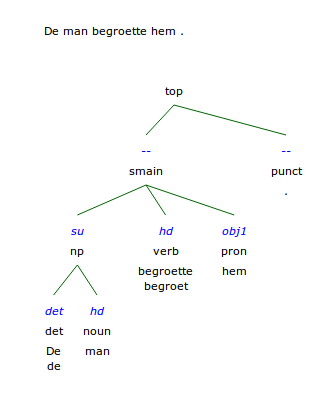
\includegraphics[width=60.0mm]{alpino.png}
\end{center}
\caption{Alpino dependency parse for the Dutch sentence ``De man begroette hem.''}
\label{fig:arch} 
\end{figure}
\FloatBarrier

\begin{lstlisting}[language=xml]
<s xml:id="example.p.1.s.1">
  <t>De man begroette hem.</t>
  <w xml:id="example.p.1.s.1.w.1"><t>De</t></w>
  <w xml:id="example.p.1.s.1.w.2"><t>man</t></w>
  <w xml:id="example.p.1.s.1.w.3"><t>begroette</t></w>
  <w xml:id="example.p.1.s.1.w.4"><t>hem</t></w>
  <w xml:id="example.p.1.s.1.w.5"><t>.</t></w>
  <syntax set="http://ilk.uvt.nl/folia/sets/alpino">
    <su xml:id="example.p.1.s.1.su.1" class="top">     
        <su xml:id="example.p.1.s.1.su.1_1" class="smain">     
            <su xml:id="example.p.1.s.1.su.1_1_1" class="np">     
                <su xml:id="example.p.1.s.1.su.1_1_1_1" class="top">     
                    <wref id="example.p.1.s.1.w.1" t="De" />       
                </su>
                <su xml:id="example.p.1.s.1.su.1_1_1_2" class="top">     
                    <wref id="example.p.1.s.1.w.2" t="man" />
                </su> 
            </su>
            <su xml:id="example.p.1.s.1.su.1_1_2" class="verb">     
                <wref id="example.p.1.s.1.w.3" t="begroette" />   
            </su>
            <su xml:id="example.p.1.s.1.su.1_1_3" class="pron">     
                <wref id="example.p.1.s.1.w.4" t="hem" />   
            </su>
        </su>
        <su xml:id="example.p.1.s.1.su.1_2" class="punct">
            <wref id="example.p.1.s.1.w.5" t="." />               
        </su> 
    </su>
  </syntax>
  <dependencies>
    <dependency xml:id="example.p.1.s.1.dependency.1" class="det">
        <hd su="example.p.1.s.1.su.1_1_1_2">
           <wref id="example.p.1.s.1.w.2" t="man" />   
        </hd>
        <dep ref="example.p.1.s.1.su.1_1_1_1">
            <wref id="example.p.1.s.1.w.1" t="De" />   
        </dep>
    </dependency>
    <dependency xml:id="example.p.1.s.1.dependency.2" class="obj1">
        <hd su="example.p.1.s.1.su.1_1_2">
            <wref id="example.p.1.s.1.w.3" t="begroette">
        </hd>
        <dep su="example.p.1.s.1.su.1_1_3">
            <wref id="example.p.1.s.1.w.4" t="hem" />   
        </dep>
    </dependency>
  </dependencies>
</s>
\end{lstlisting}

The declaration:

\begin{lstlisting}[language=xml]
<annotations>
    <token-annotation set="http://ilk.uvt.nl/folia/sets/ucto-tokconfig-nl" 
     annotator="ucto" annotatortype="auto" />
    <syntax-annotation set="http://ilk.uvt.nl/folia/sets/alpino-syntax" /> 
    <dependency-annotation set="http://ilk.uvt.nl/folia/sets/alpino-dep" />
</annotations>
\end{lstlisting}

\subsection{Chunking}

Unlike a full syntactic parse, chunking is not nested. The layer for this type of linguistic annotation is predictably called \texttt{chunking}. The span annotation element itself is \texttt{chunk}.

\begin{lstlisting}[language=xml]
<s xml:id="example.p.1.s.1">
  <t>The Dalai Lama greeted him.</t>
  <w xml:id="example.p.1.s.1.w.1"><t>The</t></w>
  <w xml:id="example.p.1.s.1.w.2"><t>Dalai</t></w>
  <w xml:id="example.p.1.s.1.w.3"><t>Lama</t></w>
  <w xml:id="example.p.1.s.1.w.4"><t>greeted</t></w>
  <w xml:id="example.p.1.s.1.w.5"><t>him</t></w>
  <w xml:id="example.p.1.s.1.w.6"><t>.</t></w>
  <chunking>
    <chunk xml:id="example.p.1.s.1.chunk.1">       
        <wref id="example.p.1.s.1.w.1" t="The" />       
        <wref id="example.p.1.s.1.w.2" t="Dalai" />       
        <wref id="example.p.1.s.1.w.3" t="Lama" />        
    </chunk>
    <chunk xml:id="example.p.1.s.1.chunk.2">       
        <wref id="example.p.1.s.1.w.4" t="greeted" />
    </chunk>
    <chunk xml:id="example.p.1.s.1.chunk.3">       
        <wref id="example.p.1.s.1.w.5" t="him" />
        <wref id="example.p.1.s.1.w.6" t="." />
    </chunk>    
  </chunking>
</s>
\end{lstlisting}


The declaration:

\begin{lstlisting}[language=xml]
<annotations>
    <chunking-annotation set="http://ilk.uvt.nl/folia/sets/syntax-nl" />
</annotations>
\end{lstlisting}



\subsection{Semantic roles}

\begin{devnotes}
Still to be done.. The \texttt{semroles} layer and \texttt{semrole} span annotation element will be reserved for this.
\end{devnotes}

\subsection{Alterative Span Annotations}

With token annotations one could specify an unbounded number of alternative annotations. This is possible for span annotations as well, but due to the different nature of span annotations this happens in a slightly different way.

Where we used \texttt{alt} for token annotations, we now use \texttt{altlayers} for span annotations. Under this element several alternative layers can be presented. Analogous to \texttt{alt}, any layers grouped together are assumed to be somehow dependent. Multiple \texttt{altlayers} can be added to introduce independent alternatives. Each alternative should be associated with a unique identifier, which uses ``alt'' rather than ``altlayers''. In this case, any layers it consists of must be marked as non-autoritative using \texttt{auth="no"}.

Below is an example of a sentence that is chunked in two ways:

\begin{lstlisting}[language=xml]
<s xml:id="example.p.1.s.1">
  <t>The Dalai Lama greeted him.</t>
  <w xml:id="example.p.1.s.1.w.1"><t>The</t></w>
  <w xml:id="example.p.1.s.1.w.2"><t>Dalai</t></w>
  <w xml:id="example.p.1.s.1.w.3"><t>Lama</t></w>
  <w xml:id="example.p.1.s.1.w.4"><t>greeted</t></w>
  <w xml:id="example.p.1.s.1.w.5"><t>him</t></w>
  <w xml:id="example.p.1.s.1.w.6"><t>.</t></w>
  <chunking>
    <chunk xml:id="example.p.1.s.1.chunk.1">       
        <wref id="example.p.1.s.1.w.1" t="The" />       
        <wref id="example.p.1.s.1.w.2" t="Dalai" />       
        <wref id="example.p.1.s.1.w.3" t="Lama" />        
    </chunk>
    <chunk xml:id="example.p.1.s.1.chunk.2">       
        <wref id="example.p.1.s.1.w.4" t="greeted" />
    </chunk>
    <chunk xml:id="example.p.1.s.1.chunk.3">       
        <wref id="example.p.1.s.1.w.5" t="him" />
        <wref id="example.p.1.s.1.w.6" t="." />
    </chunk>    
  </chunking>
  <altlayers xml:id="example.p.1.s.1.alt.1">
       <chunking annotator="John Doe" 
        annotatortype="manual" confidence="0.0001" auth="no">
        <chunk xml:id="example.p.1.s.1.alt.1.chunk.1">       
            <wref id="example.p.1.s.1.w.1" t="The" />       
            <wref id="example.p.1.s.1.w.2" t="Dalai" />                       
        </chunk>
        <chunk xml:id="example.p.1.s.1.alt.1.chunk.2">       
            <wref id="example.p.1.s.1.w.2" t="Lama" />                       
            <wref id="example.p.1.s.1.w.4" t="greeted" />
        </chunk>
        <chunk xml:id="example.p.1.s.1.alt.1.chunk.3">       
            <wref id="example.p.1.s.1.w.5" t="him" />
            <wref id="example.p.1.s.1.w.6" t="." />
        </chunk>    
      </chunking>   
  </altlayers>
</s>
\end{lstlisting}

The support for alternatives and the fact that multiple layers (including those of different types) cannot be nested in a single inline structure, should make clear why FoLiA uses a stand-off notation alongside an inline notation. 



\section{Advanced Paradigm}
\label{sec:advparadigm}

We introduced the FoLiA paradigm in section~\ref{sec:paradigm}. Now we will introduce some of the more advanced aspects of the FoLiA paradigm. These are relevant especially if you want to submit suggestions for extending the FoLiA format with annotations not yet supported.

\subsection{Human readable Descriptions}

Any token annotation element or span annotation element may hold a \texttt{desc} element containing a human readable description for the annotation. An example of this has been already shown for the \texttt{sense} and \texttt{gap} elements.

\subsection{Text content and multiple classes}
\label{sec:textcontent}

In section~\ref{sec:basics} we have seen the text content element \texttt{t}. This element can be associated with structural elements such as \texttt{w}, \texttt{s}, and \texttt{p}. The \texttt{offset} attribute may be used to explicitly link the text between child and parent. This is demonstrated on three levels in the following example:

\begin{lstlisting}[language=xml]
 <p xml:id="example.p.1">
    <t>Hello. This is a sentence. Bye!</t>
    <s xml:id="example.p.1.s.1">        
        <t offset="7">This is a sentence.</t>    
        <w xml:id="example.p.1.s.1.w.1"><t offset="0">This</t></w>
        <w xml:id="example.p.1.s.1.w.2"><t offset="5">is</t></w>
        <w xml:id="example.p.1.s.1.w.3"><t offset="8">a</t></w>
        <w xml:id="example.p.1.s.1.w.4" space="no"><t offset="10" >sentence</t></w>
        <w xml:id="example.p.1.s.1.w.5"><t offset="18">.</t></w>
    </s>
 </p>
\end{lstlisting}

Moreover, we have seen the space attribute, which is a simple alternative that can be used to reconstruct the untokenised text if it is not explicitly provided in a parent's \texttt{t} element. Allowed values for \texttt{space} are:

\begin{itemize}
\item ``\texttt{yes}'' or ``\texttt{ }'' (a space) -- This is the default and says that the token is followed by a single space.
\item ``\texttt{no}'' or ``\texttt{}'' (empty) -- This states that the token is not followed by a space.
\item any other character or string -- This states that the token is followed by another character or string that acts as a token separator.
\end{itemize}


When explicit text content on sentence/paragraph level is provided, offsets can be used to refer back to it from deeper text-content elements. This does imply that there are some challenges to solve. First of all, by default, the offset refers to the direct parent of whatever element the text content (\texttt{t}) is a member of. If a level is missing we have to explicitly specify this reference using the \texttt{ref} attribute. Note that there is no text content for the sentence in the following example, and we refer directly to the paragraph's text:

\begin{lstlisting}[language=xml]
 <p xml:id="example.p.1">
    <t>Hello. This is a sentence. Bye!</t>
    <s xml:id="example.p.1.s.1">        
        <w xml:id="example.p.1.s.1.w.1">
         <t ref="example.p.1" offset="7">This</t>
        </w>
        <w xml:id="example.p.1.s.1.w.2">
         <t ref="example.p.1" offset="12">is</t>
        </w>
        <w xml:id="example.p.1.s.1.w.3">
         <t ref="example.p.1" offset="15">a</t>
        </w>
        <w xml:id="example.p.1.s.1.w.4" space="no">
         <t ref="example.p.1" offset="17">sentence</t>
        </w>
        <w xml:id="example.p.1.s.1.w.5">
         <t ref="example.p.1" offset="25">.</t>
        </w>
    </s>
 </p>
\end{lstlisting}

Note that text content is always expected to be untokenised, except in \texttt{w} tags as it by definition is the tokenisation layer.

It is possible to associate \emph{multiple text-content} elements with the same element, and thus associating multiple texts with the same element. You may wonder what could possibly be the point of such extra complexity. But there is a clear use-case when dealing with for example corrections, or wanting to associate the text version just prior or after a processing step such as Optical Character Recognition or another kind of normalisation.

Corrections are challenging because they can be applied to text content and thus change the text. Corrections are often applied on the token level (within \texttt{w} tags), but you may want them propagated to the text content of sentences or paragraphs whilst at the same time wanting to retain the text how it originally was. This can be accomplished by introducing text content of a different class. Text content that has no associated class obtains the ``current'' class by default, it is expected to always be up-to-date. There is a notable exception: text content that appears within the scope of \texttt{original} elements within a \texttt{correction} element automatically adopts the ``original'' class.\footnote{For more deeply nested original elements, you will have to assign your own classes if you do not want them to take the ``original'' class.} This thus implies that in this rare case, FoLiA actually pre-defines classes (i.e: ``original'' and ``current'')! In addition to these two pre-defined classes, any other custom classes may be added as you see fit. If you add custom classes, you need a declaration:

\begin{lstlisting}[language=xml]
<annotations>
    <text-annotation set="http://ilk.uvt.nl/folia/sets/text-annotation" />
</annotations>
\end{lstlisting}


Below is an example illustrating the usage of multiple classes. To show the flexibility, offsets are added, but these are of course always optional. Note that when an offset is specified, it always refers to a text-content element of the same class! 
%Whenever a text content element has an associated class, it also needs to be marked as non-authoritative using \texttt{auth="no"}. This facilitates the job of parsers seeking to extract the mo

\begin{lstlisting}[language=xml]
 <p xml:id="example.p.1">
    <t>Hello. This is a sentence. Bye!</t> 
    <t class="original">Hello. This iz a sentence. Bye!</t>    
    <s xml:id="example.p.1.s.1">        
        <t offset="7">This is a sentence.</t>
        <t class="original" offset="7">This is a sentence.</t>
        <w xml:id="example.p.1.s.1.w.1">
         <t offset="0">This</t>
        </w>
        <w xml:id="example.p.1.s.1.w.2">         
         <correction>
          <new>
           <t offset="5">is</t>
          </new>
          <original auth="no">
           <t offset="5">iz</t> 
           <!-- Note that this element has class 'original' by definition! -->
          </original>
         </correction>
        </w>
        <w xml:id="example.p.1.s.1.w.3">
         <t offset="8">a</t>
        </w>
        <w xml:id="example.p.1.s.1.w.4" space="no">
         <t offset="10">sentence</t>
        </w>
        <w xml:id="example.p.1.s.1.w.5">
         <t offset="48">.</t>
        </w>
    </s>
 </p>
\end{lstlisting}

One important aspect is that FoLiA dictates that \texttt{t} elements without classes always appear first, before any other text-content tags that do specify classes. This rule facilitates the job of parsers in quickly getting the latest text content even if there are multiple classes: the first \texttt{t} element will be the most recent by definition.

In the above example, the correction is explicit, in the next example, it is implicit. Furthermore, to illustrate how you could use other custom classes, the next example introduces an custom ``ocroutput'' class that shows the (fictious) output of an OCR system prior to some implicit correction stage. 

\begin{lstlisting}[language=xml]
 <p xml:id="example.p.1">
    <t>Hello. This is a sentence. Bye!</t> 
    <t class="original">Hello. This iz a sentence. Bye!</t>    
    <t class="ocroutput">Hell0 Th1s iz a sentence, Bye1</t>    
    <s xml:id="example.p.1.s.1">        
        <t offset="7">This is a sentence.</t>
        <t class="original" offset="7">This is a sentence.</t>
        <t class="ocroutput" offset="6">Th1s iz a sentence,</t>
        <w xml:id="example.p.1.s.1.w.1">
         <t offset="0">This</t>
         <t class="ocroutput" offset="0">Th1s</t>
        </w>
        <w xml:id="example.p.1.s.1.w.2">         
           <t offset="5">is</t>
           <t offset="5" class="original">iz</t> 
           <t offset="5" class="ocroutput">iz</t>           
        </w>
        <w xml:id="example.p.1.s.1.w.3">
         <t offset="8">a</t>
        </w>
        <w xml:id="example.p.1.s.1.w.4" space="no">
         <t offset="10">sentence</t>
        </w>
        <w xml:id="example.p.1.s.1.w.5">
         <t offset="48">.</t>
         <t offset="48" class="original">.</t>
         <t offset="48" class="ocroutput">,</t>
        </w>
    </s>
 </p>
\end{lstlisting}



Last, an important note regarding offsets; all offset values are measured in unicode code-points, the first character having index zero. Take special care with combining diacritical marks versus codepoints that directly integrate the diacritical mark.

\subsection{Subsets and multiple classes}
\label{subset}

For some annotations, associating a single class from a set is not sufficient. FoLiA provides the option to associate multiple classes, or to associate classes with specific subsets. 


Take a look at the following abstract case: \texttt{X} here is a \emph{fictional} token/span annotation. It is associated with two classes from the same set. The fictional element \texttt{Y} goes with \texttt{X}, and is custom to the specific annotation.

\begin{lstlisting}[language=xml]
<X set="a">
    <Y class="p">
    <Y class="q">
</X>
\end{lstlisting}

The classes can be made members of a certain subset, rather than the main set. Subsets are assumed to in turn defined by the main set. No special declarations will be necessary.

\begin{lstlisting}[language=xml]
<X set="a">
    <Y subset="f" class="p">
    <Y subset="g" class="q">
</X>
\end{lstlisting}

Optionally, \texttt{X} itself might also be associated with a class, the class in this case would either represent all sub-parts, \emph{or} be the basis upon which redefinement is made. Which of the two is chosen depends on the set used.

FoLiA has a default element \texttt{feat} that can be used instead of \texttt{Y} in the last-mentioned example above, so that no special elements needs to be introduced. This \texttt{feat} element can always be used to freely to associate \texttt{any} additional classes of \emph{any} designed subset with with \emph{any} annotation element !!!

If elements such as the ficticious \texttt{Y} are introduced then they can be implicitly associated with a specific subset:

\begin{lstlisting}[language=xml]
<X set="a" class="p">
    <Y class="q">
</X>
\end{lstlisting}

In such cases, if a subset is implied and there can be only one instance, a more common and concise solution would be to add \texttt{Y} as an attribute:

\begin{lstlisting}[language=xml]
<X set="a" class="p" y="q" />
\end{lstlisting}

An example of this is seen in the \texttt{sense} element, which takes a \texttt{synset} attribute that is implicitly associated with a subset of synsets.

\begin{lstlisting}[language=xml]
<sense class="p" synset="q" />
\end{lstlisting}

A second example is the \texttt{event} element with the \texttt{actor} attribute:

\begin{lstlisting}[language=xml]
<event class="p" actor="q">
\end{lstlisting}

FoLiA implicitly relates the synset attribute here to the ``synset'' subset of whatever set you defined. Note that any such implicit subset relation needs to be defined by the FoLiA standard itself, you can't just make up such attributes yourself. This section mainly served to gain insight in the advanced aspects of FoLiA, and to be able to suggest additions to it that follow the same principles.

\subsection{Part-of-Speech tags with features}
\label{sec:posfeat}

Part-of-speech tags are a good example of the scenario outlined above. Part-of-speech tags may consist of multiple features, which in turn \emph{may} be associated with specific subsets. There are two scenarios envisionable, one in which the class of the \texttt{pos} element combines all features, and one in which it is the foundation upon which is expanded. Which one is used is entirely up to the defined set.

Option one:

\begin{lstlisting}[language=xml]
<w xml:id="example.p.1.s.1.w.2">
    <t>boot</t>
    <pos head="N" class="N(soort,ev,basis,zijd,stan)">
        <desc>Noun, singular, neuter</desc>
        <feat subset="ntype" class="soort" />
        <feat subset="number" class="ev" />
        <feat subset="degree" class="basis" />
        <feat subset="gender" class="zijd" />
        <feat subset="case" class="stan" />
    </pos>
</w>
\end{lstlisting}

In FoLiA, this attribute \texttt{head} is implicitly associated with the subset ``head'' of whatever set you defined.

Option two:

\begin{lstlisting}[language=xml]
<w xml:id="example.p.1.s.1.w.2">
    <t>boot</t>
    <pos class="N">
        <desc>Noun, singular, neuter</desc>
        <feat subset="ntype" class="soort" />
        <feat subset="number" class="ev" />
        <feat subset="degree" class="basis" />
        <feat subset="gender" class="zijd" />
        <feat subset="case" class="stan" />
    </pos>
</w>
\end{lstlisting}


\section{Subtoken Annotation}

Subtoken category combines aspects from both token annotation and span annotation. It introduces an annotation layer at the token level, as child of the \texttt{w} element. Within this annotation layer, subtoken annotation elements can be used to annotate parts within the token itself. Whereas span elements use \texttt{wref} to refer to words, subannotation elements use \texttt{t} to refer to part of the text of the token. Recall that \texttt{t} elements can contain references to higher-level \texttt{t} elements. In such cases, the \texttt{offset} attribute is used to designate the offset index in the word's associated text element (\texttt{t}) (zero being right at the start of the text).

\subsection{Morphological Analysis}


\begin{lstlisting}[language=xml]
<w xml:id="example.p.4.s.2.w.4">
    <t>leest</t>
    <lemma class="lezen" />
    <morphology>
        <morpheme>
            <feat subset="type" class="stem">
            <feat subset="function" class="lexical">
            <t offset="0">lees</t>
        </morpheme>
        <morpheme>
            <feat subset="type" class="suffix">
            <feat subset="function" class="inflexional">
            <t offset="4">t</t>
        </morpheme>
    </morphology>
</w>
\end{lstlisting}


\begin{lstlisting}[language=xml]
<annotations>
    <morphology-annotation set="http://ilk.uvt.nl/folia/sets/entities" />
</annotations>
\end{lstlisting}

\subsection{Named Entities within a token}

Named entities may sometimes occur as \emph{part} of a token. The \texttt{subentities} annotation layer and the \texttt{subentity} subtoken annotation element can be used for annotating these:  

\begin{lstlisting}[language=xml]
<w xml:id="example.p.4.s.2.w.4">
    <t>CDA-voorzitter</t>
    <subentities>
        <subentity class="org" annotator="Maarten van Gompel"
            annotatortype="manual">
            <t offset="0">CDA</t>
        </subentity>
    </subentities>
</w>
\end{lstlisting}

The declaration:

\begin{lstlisting}[language=xml]
<annotations>
    <subentity-annotation set="http://ilk.uvt.nl/folia/sets/entities" />
</annotations>
\end{lstlisting}


\section{Alignments}

FoLiA provides a facility to align parts of your document with other parts of your document, or even with parts of other FoLiA documents. These are called \emph{alignments} and are implemented using either the \texttt{alignment} element, a form of extended token annotation (that may thus also be applied on other levels such as sentences or paragraphs), or \texttt{complexalignment}, a form of span annotation for more complex word alignments.

Consider the following two aligned sentences from two \emph{distinct} FoLiA documents in different languages. Note that the \texttt{t} attribute to the \texttt{aref} element is merely optional and is this overhead is added simply to facilitate the job of limited FoLiA parsers and providing a quick reference to the target text for both parser and human user. The \texttt{xlink:href} argument is used to link to the target document, if any. If the alignment is within the same document then it should be simply omitted.

\begin{lstlisting}[language=xml]
<s xml:id="example-english.p.1.s.1">
  <t>The Dalai Lama greeted him.</t>
  <alignment class="french-translation" xlink:href="doc-french.xml" 
    xlink:type="simple">
     <aref id="doc-french.p.1.s.1" t="Le Dalai Lama le saluait." />
  </alignment>
</s>

<s xml:id="example-french.p.1.s.1">
  <t>Le Dalai Lama le saluait.</t>
  <alignment class="english-translation" xlink:href="doc-english.xml" 
    xlink:type="simple">
      <aref id="doc-english.p.1.s.1" t="The Dalai Lama greeted him." />
  </alignment>
  <alignment class="english-translation" xlink:href="doc-dutch.xml" 
     xlink:type="simple">
      <aref id="doc-dutch.p.1.s.1" t="De Dalai Lama begroette hem." />
  </alignment>
</s>
\end{lstlisting}


Although the above example has a single alignment reference (\texttt{aref}), it is not forbidden to link to specify multiple references within the \texttt{alignment} block. For more complex alignments however, such as word alignments that include many-to-one, one-to-many or many-to-many alignments, the span annotation element \texttt{complexalignment} may be more suitable. The following example illustrates a many-to-many word-alignment of the word ``Dalai Lama'' from English to French. This takes places within the \texttt{complexalignments} annotation layer.

\begin{lstlisting}[language=xml]
<s xml:id="example-english.p.1.s.1">
  <t>The Dalai Lama greeted him.</t>
  <w xml:id="example-english.p.1.s.1.w.1"><t>The</t></w>
  <w xml:id="example-english.p.1.s.1.w.2"><t>Dalai</t></w>
  <w xml:id="example-english.p.1.s.1.w.3"><t>Lama</t></w>
  <w xml:id="example-english.p.1.s.1.w.4"><t>greeted</t></w>
  <w xml:id="example-english.p.1.s.1.w.5"><t>him</t></w>
  <w xml:id="example-english.p.1.s.1.w.6"><t>.</t></w>
  <complexalignments>
        ...
    <complexalignment class="french-translation" xlink:href="doc-french.xml"
          xlink:type="simple">
        <wref id="example-english.p.1.s.1.w.2" t="Dalai">
        <wref id="example-english.p.1.s.1.w.3" t="Lama">
        <aref id="example-french.p.1.s.1.w.2" t="Dalai">
        <aref id="example-french.p.1.s.1.w.3" t="Lama">
    </complexalignment>
        ...
  </complexalignments>
</s>
\end{lstlisting}

\section{Metadata}

FoLiA has support for metadata, most notably the extensive and mandatory declaration section for all used annotations which you have seen throughout this documentation. To complement this, there is FoLiA's native metadata system, in which simple metadata fields can be defined and used at will. FoLiA is also able to operate with IMDI or CMDI metadata, either in external file or stored inline. Note however that storing CMDI or IMDI inside your FoLiA document may cause problems when you want to validate your FoLiA document. It is also incompatible with CMDI or IMDI editors that are unaware of FoLiA.

Reference to CMDI in external file proceeds in the following simple fashion:

\begin{lstlisting}[language=xml]
<metadata type="cmdi" src="/path/or/url/to/metadata.cmdi">
 ...
</metadata>
\end{lstlisting}

The procedure for IMDI is the same:

\begin{lstlisting}[language=xml]
<metadata type="imdi" src="/path/or/url/to/metadata.imdi">
 ...
</metadata>
\end{lstlisting}

If you use neither CMDI nor IMDI, then you can use FoLiA's native system, which is very simple: It introduces the \texttt{meta} element that allows you to define key value pairs as follows:

\begin{lstlisting}[language=xml]
<metadata type="native">
    <annotations>
    ..
    </annotations>
    <meta id="title">Title to my document</meta>
    <meta id="language">eng</meta>
</metadata>
\end{lstlisting}

You can simply define fields with custom IDs, but the following fields are pre-defined and recommended to be filled:

\begin{itemize}
\item \textbf{title} -- The title of the FoLiA document
\item \textbf{language} -- An ISO-639-3 language code identifying the language the document is 
\item \textbf{date} -- The date of publication in \texttt{YYYY-MM-DD} format
\item \textbf{publisher} -- The publishing institution or individual
\item \textbf{license} -- The type of license of the document (for example: \emph{GNU Free Documentation License})
\end{itemize}



\chapter{Set Definition Format}

\section{Introduction}

The FoLiA format consists not just out of the Document Format discussed in the previous chapter, but also of a Set Definition Format. The document format is agnostic about all sets and the classes therein, it is the Set Definition Format that defines precisely what classes are allowed in a set, including any subsets.

Recall from section~\ref{declarations} that all used sets need to be declared in the document and that they point to URLs holding a FoLiA set definition. If no set definition files are associated, then a full in-depth validation can not take place.

\section{Types and classes}

The set definition format is fairly straightforward, each set definition file represents one set, including all of its subsets.

Here is a simple example:

\begin{lstlisting}[language=xml]
<set xml:id="simplepos" type="closed">
    <class xml:id="N" label="Noun" />
    <class xml:id="V" label="Verb" />
    <class xml:id="A" label="Adjective" />
</set>
\end{lstlisting}

The \texttt{ID} of the class is the value that may be used in the \texttt{class} attribute in the FoLiA document. The \texttt{label} attribute carries a human readable description for presentational purposes, this is optional but highly recommended.

There are three possible types for sets and subsets: 

\begin{enumerate}
\item \textbf{open}: classes may be anything and are not defined
\item \textbf{closed}: classes are defined
\item \textbf{mixed}: classes may be anything, but some are predefined
\end{enumerate}

A set definition file for an open type set definition may be as concise as:

\begin{lstlisting}[language=xml]
<set xml:id="lemmas-nl" type="open" />
\end{lstlisting}

\section{Concept link}

You may want to associate classes, or even sets themselves, with some kind of semantic web or category registry. This link can be made using the \texttt{conceptlink} attribute which may be placed on classes, sets and subset elements. 

\begin{lstlisting}[language=xml]
<set xml:id="simplepos" type="closed" conceptlink="http://some/host/simplepos">
    <class xml:id="N" label="Noun" conceptlink="http://some/host/noun" />
    <class xml:id="V" label="Verb" conceptlink="http://some/host/verb" />
    <class xml:id="A" label="Adjective" conceptlink="http://some/host/adj" />
</set>
\end{lstlisting}

FoLiA does not dictate any format requirements for conceptual links, it can be anything, such as an RDF resource, or any other kind. If you want something more specific, or you want to link to multiple semantic resources, simply use your own ``conceptlink'' attribute in different custom XML namespace.

\section{Subsets}

Section~\ref{subset} introduced subsets. These can be defined in a similar fashion to sets and also carry a \texttt{type} attribute:

\begin{lstlisting}[language=xml]
<set xml:id="simplepos" type="closed">
    <class xml:id="N" label="Noun" />
    <class xml:id="V" label="Verb" />
    <class xml:id="A" label="Adjective" />   
    <subset xml:id="gender" class="closed">
        <class xml:id="m" label="Masculine" />    
        <class xml:id="f" label="Feminine" />
        <class xml:id="n" label="Neuter" />
    </subset>
</set>
\end{lstlisting}

It is possible for subsets to be used multiple times if the subset is declared with the attribute \texttt{multi} set to \texttt{true} (defaults to false). This allows multiple classes to be associated with a subset.

\section{Constraints}

Not all classes in subsets can be combined with others. There is the need to put constraints on which may go together. The previous example already illustrates this. For many languages, the ``gender'' subset does not make sense on verbs. We can put a constaint on the usage of this subset, limiting its usage to nouns and adjectives:

\begin{lstlisting}[language=xml]
<set xml:id="simplepos" type="closed">
    <class xml:id="N" label="Noun" />
    <class xml:id="V" label="Verb" />
    <class xml:id="A" label="Adjective" />   
    <subset xml:id="gender" class="closed">
        <constraint>
            <restrict class="N" />
            <restrict class="A" />
        </constraint>
        <class xml:id="m" label="Masculine" />    
        <class xml:id="f" label="Feminine" />
        <class xml:id="n" label="Neuter" />
    </subset>
</set>
\end{lstlisting}

For sake of brevity, constraints can be named and referred to when they are needed multiple times.

\begin{lstlisting}[language=xml]
<set xml:id="simplepos" type="closed">
    <class xml:id="N" label="Noun" />
    <class xml:id="V" label="Verb" />
    <class xml:id="A" label="Adjective" />   
    <subset xml:id="gender" class="closed">
        <constraint name="constraint.1">
            <restrict class="N" />
            <restrict class="A" />
        </constraint>
        <class xml:id="m" label="Masculine" />    
        <class xml:id="f" label="Feminine" />
        <class xml:id="n" label="Neuter" />
    </subset>
    <subset xml:id="case" class="closed">
        <constraint ref="constraint.1" />
        <class xml:id="nom" label="Nominative" />    
        <class xml:id="gen" label="Genitive" />
        <class xml:id="dat" label="Dative" />
        <class xml:id="acc" label="Accusative" />
    </subset>
</set>
\end{lstlisting}

Constraints can be used within subsets, but also within classes:

\begin{lstlisting}[language=xml]
<set xml:id="simplepos" type="closed">
    <class xml:id="N" label="Noun" />
    <class xml:id="V" label="Verb" />
    <class xml:id="A" label="Adjective" />   
    <subset xml:id="gender" class="closed">
        <class xml:id="m" label="Masculine">
            <constraint name="constraint.1">
                <restrict class="N" />
                <restrict class="A" />
            </constraint>
        </class>    
    </subset>
</set>
\end{lstlisting}

Using the restrict element, you force a certain class from the main set or any subset, thus enumerating all the allowed classes. For example, the follow constraint demands masculine or feminine noun in either nominative or accusative case. All of the restrictions must be satisfied for the constraint to match.

\begin{lstlisting}[language=xml]
<constraint>
    <restrict class="N" />
    <restrict subset="gender" class="f" />
    <restrict subset="gender" class="m" />
    <restrict subset="case" class="nom" />
    <restrict subset="case" class="acc" />
</constraint>
\end{lstlisting}

You can also opt to specify the ``forbidden'' classes using except. Only if not a single one of the exceptions applies, the constraint is met. 

\begin{lstlisting}[language=xml]
<constraint>
    <except class="V" />
    <except class="A" />
    <except subset="gender" class="n" />
    <except subset="case" class="gen" />
    <except subset="case" class="dat" />
</constraint>
\end{lstlisting}

Restrict and except elements can also be mixed.


\appendix
\chapter{Common Queries}

Considering the fact that FoLiA is an XML-based format, XPath and its derivatives are the designated tools for searching in a FoLiA document.

A very common XPath predicate found in many XPath expressions for FoLiA is \texttt{not(ancestor-or-self::*/@auth)}. This exploits the notion of authoritativeness. Certain elements in FoLiA are non-authoritative, which means that they have no direct bearing on the actual state of the element they describe. The most notable elements that are non-authorititive are alternatives, suggestions for correction, and the original part of a correction. The predicate \texttt{not(ancestor-or-self::*/@auth)} guarantees that no elements can be selected that occur within the scope of any non-authoritive element. This prevents selecting for example alternative annotations or annotations that were superseded by a correction step. This is in most cases what the user wants and why you will find this predicate appended to almost every XPath expression for FoLiA.

Some common XPath queries are listed below, note that for brevity and readability the namespace prefix is omitted. In actual situations you will have to specify the FoLiA namespace with each element, as XPath unfortunately has no notion of a default namespace.

\begin{itemize}
\item XPath query for all paragraphs: \texttt{//p[not(ancestor-or-self::*/@auth)]}
\item XPath query for all sentences: \texttt{//s[not(ancestor-or-self::*/@auth) and not(ancestor::quote)]} \\
    \emph{Explanation: When selecting sentences, you often do not want sub-sentences that are part of a quote, since they may overlap with the larger sentence they form a part of. The \texttt{not(ancestor::quote)} predicate guarantees this can not happen.}
\item XPath query for all words: \texttt{//w[not(ancestor-or-self::*/@auth)]}
\item XPath query for the text of all words/tokens: \texttt{//w//t[not(ancestor-or-self::*/@auth)][1]/text()} \\
    \emph{Explanation: The \texttt{[1]} predicate is important here and makes sure to select only the first text content element in case there are multiple. Recall that FoLiA dictates that the classless text element appears before any others, ensuring that this is the proper way to obtain the most recent text of an element. (See Section~\ref{sec:textcontent}}.    
\item XPath query for all words with lemma X: \texttt{//w[.//lemma[@class="X" and not(ancestor-or-self::*/@auth)] ]}
    \emph{Note: This query assumes there is only one declaration for lemma annotation, and the set has been verified}
\item XPath query for all words with PoS-tag A in set S: \texttt{//w[.//pos[@set="S" and @class="A" and not(ancestor-or-self::*/@auth)] ]}
    \emph{Note: This query assumes the set attribute was set explicitly, i.e. there are multiple possible sets in the document for this annotation type}
\item XPath query for the text of all words with PoS-tag A in set S: \texttt{//w[.//pos[@set="S" and @class="A" and not(ancestor-or-self::*/@auth)] ]//t[not(ancestor-or-self::*/@auth)][1]/text()}
    \emph{Note: The predicate for non-authoritativeness here needs to be applied both to the pos element and the text content element \texttt{t}, otherwise you may accidentally select the text of words which have the desired pos tag only as an alternative.}
\item XPath query to select all alternative PoS tags for all words: \texttt{//w/alt/pos} \\       
\end{itemize}

Before you release XPath queries on FoLiA documents, make sure to first parse the declarations present in the metadata (the \texttt{annotations} block). Verify that the annotation type with the desired set you are looking for is actually present, otherwise you needn't bother running a query at all. Note that the XPath expression differs based on whether there is only one set defined for the sought annotation type, or if there are multiple. In the former case, you can't use the @set attribute to select, and in the latter case, you must.

\chapter{Validation}

Validation proceeds at two levels: shallow validation and deep validation. Shallow validation considers only the structure of the FoLiA document, without validating the sets and classes used. Deep validation checks the sets and classes for their validity using the set definition files.

Shallow validation is performed using a RelaxNG schema, to be found at \texttt{https://github.com/proycon/folia/blob/master/schemas/folia.rng} .

You can validate your document using standard XML tools such as \texttt{xmllint} or \texttt{jing}, the latter is known to produce friendlier error output in case of validation errors.

\begin{lstlisting}
> xmllint -relaxng folia.rng document.xml
> jing folia.rng document.xml
\end{lstlisting}


\begin{devnotes}
Deep validation is still being worked on and will most likely use Schematron.
\end{devnotes}

\chapter{Implementations}

The following FoLiA implementations exist currently, both follow a highly object-oriented model in which FoLiA XML elements correspond with classes.

\begin{enumerate}
\item \texttt{pynlpl.formats.folia} - A FoLiA library in Python. Part of the Python Natural Language Processing Library. Documentation can can be found at http://ilk.uvt.nl/folia/
\item \texttt{libfolia} - A FoLiA library in $C++$. (Still under heavily development, September 2011)
\end{enumerate}

The following table shows the level of FoLiA support in these libraries:

\begin{tabular}{|r|c|c|}
\hline
                        & PyNLPl & libfolia  \\
                        & python & $C++$ \\
\hline
Token Annotation        & yes & yes \\
Span Annotation         & yes & yes \\
Subtoken Annotation     & yes & yes \\
Subset/feature support  & yes & yes \\
Alternatives            & yes & yes \\
Correction Annotation   & yes & yes \\
Alignments              & not yet & not yet \\
Text offset support     & incomplete\footnote{has to be more thorougly tested} & incomplete \\
Native metadata         & yes & unknown \\
\hline
Query facility (findwords) & partial\footnote{only for token annotation} & partial\footnote{in progress} \\
\hline
IMDI metadata           & partial\footnote{can be included safely, but only a very small subset is actually interpreted} & ? \\
CMDI metadata           & no\footnote{but can be included safely, just not interpreted by library} & no \\
RelaxNG schema generation & yes\footnote{The RelaxNG schema is generated dynamically by the library itself} & no \\
RelaxNG validation      & yes & no \\
Set definition support  & partial\footnote{under development} & no \\
Deep validation (Schematron)  & not yet & no \\
D-Coi read compatibility      & partial\footnote{only basic elements, no List, Figure, etc..} & no \\
\hline
\end{tabular}

\chapter{Conversions}
 
\begin{tabular}{|l|l|l|}
\hline
from & to & status  \\
\hline
D-Coi & FoLiA & yes, via XSLT or \texttt{pynlpl.formats.folia}\footnote{via library only with basic elements, no List, Figure, etc..} \\
FoLiA & D-Coi & yes, via XSLT \footnote{With inevitable data loss for constructs that can not be represented in D-Coi} \\
Frog/Tadpole columned format & FoLiA & yes, using Python script and library \\
FoLiA & Frog/Tadpole columned format,CSV  & yes, using Python script and library \\
Alpino & FoLiA & not yet \\
FoLiA & Alpino & not yet \\
\hline
\end{tabular} 

\bibliographystyle{plain}
\bibliography{folia}


\end{document}
